\chapter{Implementierung Eye Tracker}
\label{sec:implementierung eye tracker}

\section{Einrichtung im Fahrsimulator}

<<<<<<< HEAD
Eyeware Tech hat ihren Beam Eye Tracker so aufgebaut, dass er mit handelsüblicher Hardware verwendet werden kann. Das System kann bereits mit einer handelsüblichen {\ac{USB}} Webcam oder mit einer an den Computer angeschlossenen Smartphone-Kamera eingesetzt werden. Damit die Integration des Eye Trackers in den Fahrsimulator gelingt, müssen mehrere Voraussetzungen geschaffen werden. Diese werden in den folgenden Abschnitten beschrieben. 

Die Positionierung der Kamera ist von zentraler Bedeutung. Diese soll laut Eyeware Tech mittig zum Bildschirm ausgerichtet sein \cite{lit_software_beam_eyetracker}. Die Sitzposition der Testperson hingegen muss nicht mittig zur Kamera sein. Die Testperson kann auch relativ zur Kamera links oder rechts sitzen. Diese Annahme konnte durch selbst durchgeführte Tests bestätigt werden. 
In den Eye Tracker Einstellungen müssen auch die Kameraposition und der Neigungswinkel korrekt eingestellt werden. Die genauesten Ergebnisse konnten erzielt werden, als die Kamera im Fahrsimulator mittig zur Leinwand in der Mitte des Armaturenbretts angebracht war. Die Kameraposition wurde im Eye Tracker als 'unten' und mit einem Neigungswinkel von 0° angegeben.

Grundlage für verlässliche Ergebnisse ist es, die Kalibrierung, welche der Beam Eye Tracker integriert hat, vor jeder Sitzung im Fahrsimulator durchzuführen. Insbesondere wenn mehrere Personen nacheinander fahren, die sich von ihrer Körpergröße stark unterscheiden. Die in den Beam Eye Tracker integrierte Kalibrierung besteht aus fünf Punkten, die nacheinander auf der Leinwand erscheinen. Vier Punkte werden dabei in die vier Ecken der Leinwand positioniert. Der fünfte Punkt befindet sich in der Mitte der Leinwand. Während der Kalibrierung blickt die Testperson nacheinander auf diese Punkte. Sofern die Testperson einen Punkt fest fokussiert hat, klickt sie mit der Maus auf diesen Punkt. Der Eye Tracker verknüpft dann die aktuelle Blickposition mit den Koordinaten des Punktes auf der Leinwand. Nach diesem Prinzip kalibriert sich der Eye Tracker selbst und verknüpft die Position der Pupillen mit einer Position auf der Leinwand. Wie dieser Kalibrierungsprozess im Detail funktioniert, ist nicht bekannt.

Für die Tests des Eye Trackers wurde der mittelgroße Fahrsimulator in der {\ac{HKA}} eingesetzt. Da die Leinwand sehr groß ist und das Kalibrierungsfenster des Eye Trackers nicht verkleinert werden kann, befinden sich die Kalibrierungspunkte teilweise so weit in den Ecken, dass sie vor allem unten nicht mehr auf der Leinwand angezeigt werden. Das erschwert eine präzise Interaktion. Außerdem sollten während der Kalibrierung keine großen Kopfbewegungen gemacht werden. Experimente zeigten, dass das die Tracking-Genauigkeit verringern kann. Da die Punkte durch die breite Leinwand aber außerhalb des Sichtfelds der Testperson liegen, muss diese zwangsweise eine Kopfbewegung machen. 

Eine Herangehensweise, um diese Probleme zu minimieren, ist es, die Kalibrierung immer zu zweit durchzuführen. Die Testperson ist dafür verantwortlich, auf die Kalibrierungspunkte zu schauen und die zweite Person klickt auf diese mit der Maus. Da die Punkte teilweise außerhalb des Sichtfeldes liegen und die Testperson den Kopf nicht zu sehr bewegen sollte, ist es am besten, wenn diese nicht direkt auf den jeweiligen Punkt schaut, sondern leicht daneben. Wenn der Punkt bspw. unten rechts im Eck erscheint, dann richtet die Testperson bei der Kalibrierung ihren Blick leicht versetzt nach links. Zum einen wird dadurch die Kalibrierung insgesamt verbessert, da der Kopf nicht bewegt werden muss. Zusätzlich wird dadurch ein Fehler leicht abgeschwächt, welcher durch die Krümmung der Leinwand entsteht.

Zwischenzeitlich wurde im Rahmen dieser Projektarbeit auch der Ansatz einer eigenen Kalibrierung verfolgt. Diese hat vorausgesetzt, dass der Eye Tracker bereits einmal sehr grob mit dem integrierten Kalibrierungsfenster von Beam kalibriert wurde. Bei jedem Start des Programms wurde das selbst erstellte Kalibrierungsfenster geöffnet. Allerdings war das selbst entwickelte Kalibrierungsfenster in seiner Größe anpassbar. Dadurch wurden die Punkte im Sichtfeld der Testperson angezeigt und nicht an den Rändern der Leinwand. Eine schematische Abbildung des Kalibrierungsfensters ist in Abbildung \ref{fig:eigenes_kalibrierungsfenster} zu sehen. In der Realität hatte das Fenster einen weißen Hintergrund, um die Lichtverhältnisse relativ zum Beam Kalibrierungsfenster, welches sehr dunkel ist, zu verbessern. Die Ergebnisse der Kalibrierung wurden anschließend verwendet, um die Rohdaten des Eye Trackers mit diesen zu transformieren, damit die Kalibrierung Einfluss auf die Schätzwerte der Blickposition nimmt. Die daraus resultierenden Ergebnisse wiesen allerdings keine visuell erkennbare Verbesserung auf. Auf Basis der bisherigen Ergebnisse wird daher empfohlen, die integrierte Standard-Kalibrierung des Eye Trackers zu verwenden. Der Code für die selbst entwickelte Kalibrierung ist allerdings weiterhin in auskommentierter Form vorhanden und kann bei Bedarf wieder reaktiviert und weiterentwickelt werden. 
=======
Eyeware Tech hat ihren Beam Eye Tracker so aufgebaut, dass er mit handelsüblicher Hardware verwendet werden kann. Das System kann bereits mit einer handelsüblichen {\ac{USB}} Webcam oder mit einer an den Computer angeschlossenen Smartphone-Kamera eingesetzt werden. Damit die Integration des Eye Trackers in den Fahrsimulator gelingt, müssen einige Punkte beachtet werden. 

Die Positionierung der Kamera ist von zentraler Bedeutung. Diese soll lauf Eyeware Tech mittig zum Bildschirm ausgerichtet sein \cite{lit_software_beam_eyetracker}. Die Sitzposition der Testperson hingegen muss nicht mittig zur Kamera sein. Die Testperson kann auch relativ zur Kamera weiter links oder weiter rechts sitzen. Diese Annahme konnte durch selbst durchgeführte Tests bestätigt werden. 
In den Eye Tracker Einstellungen muss auch die Kameraposition und der Neigungswinkel korrekt eingestellt werden. Die genauesten Ergebnisse konnten erzielt werden, als die Kamera im Fahrsimulator mittig auf dem Display in der Mitte des Armaturenbretts angebracht war. Die Kameraposition wurde im Eye Tracker als "unten" und mit einem Neigungswinkel von 0° angegeben.

Grundlage für verlässliche Ergebnisse ist es die Kalibrierung, welche der Beam Eye Tracker integriert hat, vor jeder Sitzung im Fahrsimulator durchzuführen. Insbesondere wenn mehrere Personen nacheinander fahren, die sich von ihrer Körpergröße stark unterscheiden. Die in den Beam Eye Tracker integrierte Kalibrierung besteht aus fünf Punkten, die nacheinander auf der Leinwand erscheinen. Vier Punkte werden dabei in die vier Ecken der Leinwand positioniert. Der fünfte Punkt befindet sich in der Mitte der Leinwand. Während der Kalibrierung blickt die Testperson nacheinander auf diese Punkte. Sofern die Testperson einen Punkt fest fokussiert hat, klickt sie mit der Maus auf diesen Punkt. Der Eye Tracker verknüpft dann die aktuelle Blickposition mit den Koordinaten des Punktes auf der Leinwand. Nach diesem Prinzip kalibriert sich der Eye Tracker selbst und verknüpft die Position der Pupillen mit einer Position auf der Leinwand. Wie dieser Kalibrierungsprozess im Detail funktioniert ist nicht bekannt.

Für die Tests des Eye Trackers wurde der mittelgroße Fahrsimulator in der {\ac{HKA}} eingesetzt. Da die Leinwand sehr groß ist und das Kalibrierungsfenster des Eye Trackers nicht verkleinert werden kann, befinden sich die Kalibrierungspunkte teilweise so weit in den Ecken, dass sie vor allem unten nicht mehr auf der Leinwand angezeigt werden. Das erschwert eine präzise Interaktion. Außerdem sollten während der Kalibrierung keine großen Kopfbewegungen gemacht werden. Experimente zeigten, dass das die Tracking Genauigkeit verringern kann. Da die Punkte durch die breite Leinwand aber außerhalb des Sichtfelds der Testperson liegen, muss diese zwangsweise eine Kopfbewegung machen. 

Eine Herangehensweise um diese Probleme zu minimieren ist es, die Kalibrierung immer zu zweit durchzuführen. Die Testperson ist dafür verantwortlich auf die Kalibrierungspunkte zu schauen und die zweite Person klickt auf diese mit der Maus. Da die Punkte teilweise außerhalb des Sichtfeldes liegen und die Testperson den Kopf nicht zu sehr bewegen sollte, ist es am besten, wenn diese nicht direkt auf den jeweiligen Punkt schaut, sondern leicht daneben. Wenn der Punkt bspw. unten rechts im Eck erscheint, dann richtet die Testperson bei der Kalibrierung ihren Blick leicht versetzt nach links. Zum einen wird dadurch die Kalibrierung insgesamt verbessert, da der Kopf nicht bewegt werden muss. Zusätzlich wird dadurch ein Fehler leicht abgeschwächt, welcher durch die Krümmung der Leinwand entsteht.
Zwischenzeitlich wurde im Rahmen dieser Projektarbeit auch der Ansatz einer eigenen Kalibrierung verfolgt. Diese hat vorausgesetzt, dass der Eye Tracker bereits einmal sehr grob mit dem integrierten Kalibrierungsfenster von Beam kalibriert wurde. Bei jedem Start des Programms wurde das selbst erstellte Kalibrierungsfenster geöffnet. Allerdings war das selbst entwickelte Kalibrierungsfenster in seiner Größe anpassbar. Dadurch wurden die Punkte im Sichtfeld der Testperson angezeigt und nicht an den Rändern der Leinwand. Eine schematische Abbildung des Kalibrierungsgfensters ist in Abbildung \ref{fig:eigenes_kalibrierungsfenster} zu sehen. In der Realität hatte das Fenster einen weißen Hintergrund, um die Lichtverhältnisse relativ zum Beam Kalibrierungsfenster, welches sehr dunkel ist, zu verbessern. Die Ergebnisse der Kalibrierung wurden anschließend verwendet, um die Rohdaten des Eye Trackers mit diesen zu transformieren, damit die Kalibrierung Einfluss auf die Schätzwerte der Blickposition nimmt. Die daraus resultierten Ergebnisse wiesen allerdings keine wirkliche Verbesserung auf. Auf Basis der bisherigen Ergebnisse wird daher empfohlen die integrierte Standard-Kalibrierung des Eye Trackers zu verwenden. Der Code für die selbst entwickelte Kalibrierung ist allerdings weiterhin in auskommentierter Form vorhanden und kann bei Bedarf wieder reaktiviert und weiterentwickelt werden. 

\begin{figure}[h]
	\begin{center}
		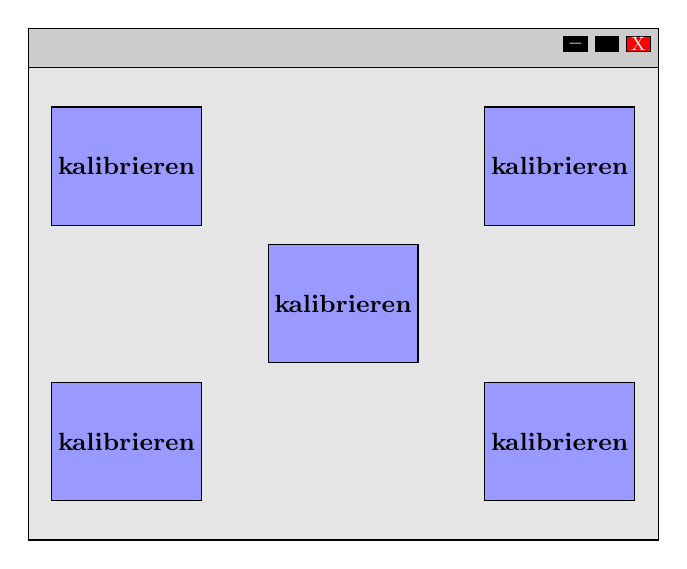
\begin{tikzpicture}[scale=1]
			% Fensterhintergrund
			\draw[fill=gray!20] (0,0) rectangle (8,6);
			
			% Fensterleiste mit Min, Max, Schließen
			\draw[fill=gray!40] (0,6) rectangle (8,6.5);
			\draw[fill=black] (6.8,6.2) rectangle (7.1,6.4); % Minimieren
			\draw[fill=black] (7.2,6.2) rectangle (7.5,6.4); % Maximieren
			\draw[fill=red] (7.6,6.2) rectangle (7.9,6.4); % Schließen
			\node at (6.95,6.3) {\textcolor{white}{\scalebox{0.7}{$-$}}};
			\node at (7.35,6.3) {\textcolor{white}{\scalebox{0.7}{$\square$}}};
			\node at (7.75,6.3) {\textcolor{white}{\scalebox{0.7}{X}}};
			
			% Kalibrierungsknöpfe
			\draw[fill=blue!40] (0.3,0.5) rectangle (2.2,2); % Unten links
			\draw[fill=blue!40] (5.8,0.5) rectangle (7.7,2); % Unten rechts
			\draw[fill=blue!40] (0.3,4) rectangle (2.2,5.5); % Oben links
			\draw[fill=blue!40] (5.8,4) rectangle (7.7,5.5); % Oben rechts
			\draw[fill=blue!40] (3.05,2.25) rectangle (4.95,3.75); % Mitte
			
			% Text auf den Knöpfen
			\node at (1.25,1.25) {\small \textbf{kalibrieren}};
			\node at (6.75,1.25) {\small \textbf{kalibrieren}};
			\node at (1.25,4.75) {\small \textbf{kalibrieren}};
			\node at (6.75,4.75) {\small \textbf{kalibrieren}};
			\node at (4,3) {\small \textbf{kalibrieren}};
		\end{tikzpicture}
	\end{center}
	\caption{Schematische Darstellung des selbst entwickelten Kalibrierungsfensters}\label{fig:eigenes_kalibrierungsfenster}
\end{figure}


Während der Kalibrierung und der gesamten Verwendung des Eye Tracking Systems darf ausschließlich die Testperson im Fahrsimulator sitzen. Eine zweite Person würde das Tracking System beeinflussen, da nicht selektiert werden kann, welche Augen getrackt werden sollen und welche nicht. In Zukunft muss hier eine visuelle Abschirmung, wie eine Art Scheuklappe eingebaut werden, um dieses Problem zu lösen. 

Ein weiterer wichtiger Faktor ist die Beleuchtung im Fahrsimulator. Das Kalibrierungsfenster des Beam Eye Trackers hat einen schwarzen Hintergrund. Wenn keine externe Lichtquelle verwendet wird, dann sind die Lichtverhältnisse unzureichend, als dass eine ordentliche Kalibrierung stattfinden könnte. Selbst wenn während der Kalibrierung gute Lichtverhältnisse herrschen, reicht die Helligkeit der Leinwand allein während des Fahrens nicht aus, um verlässliche Ergebnisse zu liefern. Es konnte eine deutliche Verbesserung der Trackingqualität erzielt werden, nachdem im Fahrsimulator eine externe Lichtquelle während der gesamten Kalibrierung und der gesamten Fahrzeit eingesetzt wurde. 
Neben externen Mitteln, um die Lichtverhältnisse zu verbessern, können auch in der Windows Kamera App Anpassungen vorgenommen werden. Dazu muss in den Einstellungen der Kamera App unter "Kameraeinstellungen" die Option "Erweiterte Steuerelemente für Fotos und Videos" aktiviert werden. Dadurch wird ein Helligkeitsregler verfügbar, der die Helligkeit des Kamerabildes systemweit verändert. Je nach aktuellen Lichtverhältnissen kann ein Erhöhen oder Verringern der Bildhelligkeit den Kontrast der Pupillen relativ zur Umgebung verbessern.

\begin{figure}[h!]
	\begin{center}
		
\includegraphics[scale=0.19]{camera_position}
		\caption{Positionierung von Kamera und externer Lichtquelle, Quelle: \cite{lit_software_canva}} \label{fig:camera_position}
	\end{center}
\end{figure}


In Abbildung \ref{fig:camera_position} sind die Kameraposition und die externe Lichtquelle aufgebaut im Fahrsimulator zu erkennen. Licht und Kamera sollten zu einem späteren Zeitpunkt noch besser in das System integriert werden. Zu Testzwecken hat der Aufbau allerdings verlässliche Ergebnisse geliefert. 
>>>>>>> fd0befd8e95e2bae230d21ece8a1862eada6b577



\begin{center}
	\resizebox{0.45\linewidth}{!}{
	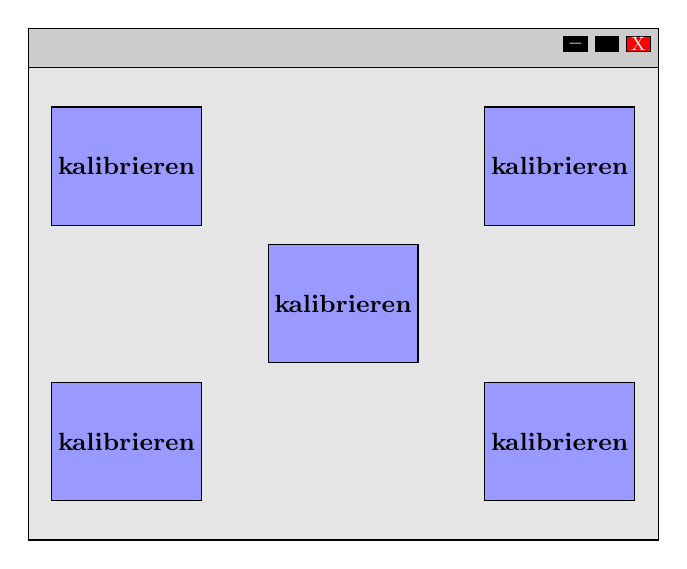
\begin{tikzpicture}[scale=1]
		% Fensterhintergrund
		\draw[fill=gray!20] (0,0) rectangle (8,6);
		
		% Fensterleiste mit Min, Max, Schließen
		\draw[fill=gray!40] (0,6) rectangle (8,6.5);
		\draw[fill=black] (6.8,6.2) rectangle (7.1,6.4); % Minimieren
		\draw[fill=black] (7.2,6.2) rectangle (7.5,6.4); % Maximieren
		\draw[fill=red] (7.6,6.2) rectangle (7.9,6.4); % Schließen
		\node at (6.95,6.3) {\textcolor{white}{\scalebox{0.7}{$-$}}};
		\node at (7.35,6.3) {\textcolor{white}{\scalebox{0.7}{$\square$}}};
		\node at (7.75,6.3) {\textcolor{white}{\scalebox{0.7}{X}}};
		
		% Kalibrierungsknöpfe
		\draw[fill=blue!40] (0.3,0.5) rectangle (2.2,2); % Unten links
		\draw[fill=blue!40] (5.8,0.5) rectangle (7.7,2); % Unten rechts
		\draw[fill=blue!40] (0.3,4) rectangle (2.2,5.5); % Oben links
		\draw[fill=blue!40] (5.8,4) rectangle (7.7,5.5); % Oben rechts
		\draw[fill=blue!40] (3.05,2.25) rectangle (4.95,3.75); % Mitte
		
		% Text auf den Knöpfen
		\node at (1.25,1.25) {\small \textbf{kalibrieren}};
		\node at (6.75,1.25) {\small \textbf{kalibrieren}};
		\node at (1.25,4.75) {\small \textbf{kalibrieren}};
		\node at (6.75,4.75) {\small \textbf{kalibrieren}};
		\node at (4,3) {\small \textbf{kalibrieren}};
	\end{tikzpicture}
}
\end{center}
\captionof{figure}{Schematische Darstellung des selbst entwickelten Kalibrierungsfensters}\label{fig:eigenes_kalibrierungsfenster}



Während der Kalibrierung und der gesamten Verwendung des Eye Tracking Systems darf ausschließlich die Testperson im Fahrsimulator sitzen. Eine zweite Person würde das Tracking System beeinflussen, da nicht selektiert werden kann, welche Augen getrackt werden sollen und welche nicht. In Zukunft muss hier eine visuelle Abschirmung, wie eine Art Scheuklappe eingebaut werden, um dieses Problem zu lösen.

Ein weiterer wichtiger Faktor ist die Beleuchtung im Fahrsimulator. Das Kalibrierungsfenster des Beam Eye Trackers hat einen schwarzen Hintergrund. Wenn keine externe Lichtquelle verwendet wird, dann sind die Lichtverhältnisse unzureichend, als dass eine ordentliche Kalibrierung stattfinden könnte. Selbst wenn während der Kalibrierung gute Lichtverhältnisse herrschen, reicht die Helligkeit der Leinwand während des Fahrens nicht aus, um verlässliche Ergebnisse zu liefern. Es konnte eine Verbesserung der Trackingqualität erzielt werden, nachdem im Fahrsimulator eine externe Lichtquelle während der gesamten Kalibrierung und der gesamten Fahrzeit eingesetzt wurde. 
Neben externen Mitteln, um die Lichtverhältnisse zu verbessern, können auch in der Windows Kamera App Anpassungen vorgenommen werden. Dazu muss in den Einstellungen der Kamera App unter 'Kameraeinstellungen' die Option 'Erweiterte Steuerelemente für Fotos und Videos' aktiviert werden. Dadurch wird ein Helligkeitsregler verfügbar, der die Helligkeit des Kamerabildes systemweit verändert. Je nach aktuellen Lichtverhältnissen kann ein Erhöhen oder Verringern der Bildhelligkeit den Kontrast der Pupillen relativ zur Umgebung verbessern.


\begin{center}
	
\includegraphics[scale=0.19]{camera_position}
	\captionof{figure}{Positionierung von Kamera und externer Lichtquelle, Quelle: \cite{lit_software_canva}} \label{fig:camera_position}
\end{center}



In Abbildung \ref{fig:camera_position} sind die Kameraposition und die externe Lichtquelle im Fahrsimulator zu erkennen. Licht und Kamera sollten zu einem späteren Zeitpunkt noch besser in das System integriert werden. Zu Testzwecken hat der Aufbau allerdings verlässliche Ergebnisse geliefert. 

\newpage

\section{Beam Eye Tracker SDK}
<<<<<<< HEAD
Eyewear Tech bietet beim Kauf des Beam Eye Tracker das {\ac{SDK}} an. Das {\ac{SDK}} ermöglicht es, die Ausgabe des Eye Trackers in selbst geschriebenen Anwendungen zu verwenden \cite{lit_website_beam_sdk_documentation}. Das {\ac{SDK}} muss nicht zusätzlich erworben werden, sondern ist im Kaufpreis des Eye Trackers enthalten.
Auf der Website des Beam {\ac{SDK}} wird in Python geschriebener Beispielcode zur Verfügung gestellt. In diesem Code werden die nötigen Schritte für eine Verbindung mit der {\ac{API}} des Eye Trackers durchgeführt. Der Code wurde auch als Grundlage für die Implementierung des Eye Trackers in dem Programm, das im Rahmen dieser Arbeit entwickelt wurde, verwendet \cite{lit_code_beam_sdk}.


\textsf{}
\begin{center}
	
\includegraphics[scale=0.11]{code_structure_beam}
	\captionof{figure}{Visuelle Darstellung des Codes zur Beam {\ac{SDK}}, Quelle: nachempfunden: \cite{lit_code_beam_sdk}, \cite{lit_software_eraserio}} \label{fig:code_structure_beam}
\end{center}



Die Funktionsweise der {\ac{API}} ist vereinfacht in Abbildung \ref{fig:code_structure_beam} zu erkennen. Der Tracker Server ist die Bezeichnung für den Eye Tracker selbst. Der Client ist das selbst geschriebene Programm, welches die Trackerdaten über die {\ac{API}} entgegennimmt. Die beiden zentralen Informationen, welche vom Server an den Client übergeben werden, sind die Daten zur Kopfposition (head pose data) und die Daten zur Blickposition (screen gaze data). Die Kopfposition gibt Auskunft über die Translation und Rotation des Kopfes der Testperson. Die Blickposition gibt Auskunft darüber, auf welchen Punkt auf dem Bildschirm die Testperson schaut \cite{lit_website_beam_sdk_documentation}. Diese beiden Systeme laufen unabhängig voneinander und dienen unterschiedlichen Einsatzzwecken. Das Kopftracking kann bspw. dazu dienen, die Kamera in einer Simulationswelt zu bewegen. Das könnte Sinn machen, wenn keine große Leinwand wie im Fahrsimulator vorhanden ist. Durch einen Blick nach links könnte sich auch die Kamera im Fahrsimulator mit nach links bewegen. Für den Einsatzzweck im Fahrsimulator ist diese Funktion durch die große Leinwand allerdings nicht notwendig. Die Daten werden dennoch übermittelt, falls in Zukunft doch ein Anwendungsfall entstehen sollte. Die Gaze Daten stellen im Kontext dieser Arbeit die primär relevante Information dar. Diese geben eine Schätzung ab, auf welchen Punkt die Testperson auf der Leinwand schaut. Sofern eine Testperson vom Eye Tracker erkannt wird, werden in kontinuierlichen Abständen diese Daten vom Eye Tracker an den Client übermittelt. Zusätzlich dazu werden auch noch andere Daten wie bspw. die confidence übermittelt. Dabei handelt es sich um einen Wert, welcher mit jeder geschätzten Blickposition mit übermittelt wird. Dieser gibt an, wie sicher sich der Eye Tracker mit seiner Schätzung der aktuellen Blickposition ist \cite{lit_website_beam_sdk_documentation}. 

\section{Schnittstelle zu CARLA}

Im folgenden Abschnitt soll der Datenfluss zwischen CARLA und dem Eye Tracker sowie dem selbstgeschriebenen Programm erläutert werden.
Der Eye Tracker und CARLA arbeiten größtenteils getrennt voneinander. Die visuelle Ausgabe des Eye Trackers erfolgt durch einen kleinen schwarzen Punkt, welcher die aktuell geschätzte Blickposition auf der Leinwand anzeigt. Dieser schwarze Punkt befindet sich in einem selbst erstellten transparenten Fenster, welches über den Bildschirm gelegt wird. Der schwarze Punkt ist nicht Teil von CARLA oder dem Eye Tracker sondern wird durch das selbst geschriebene Programm erzeugt. Er basiert auf den x- und y-Koordinaten des Eye Trackers, welche durch eine zusätzliche Korrekturfunktion optimiert werden. Diese Korrektur wird in einem späteren Abschnitt genauer erläutert. Es gibt auch einen sogenannten Textmanager. Dieser ist auch selbst entwickelt und weder Teil von CARLA noch vom Beam Eye Tracker. In diesem werden für den Nutzer unter anderem die grobe Blickrichtung in Textform angezeigt. Zum Beispiel 'schaut nach oben links'. Der Text Manager, wird wie in der Abbildung \ref{fig:eye_tracker_data} zu sehen ist, mit Informationen des Eye Trackers und von CARLA gespeist.

Die einzige direkte Schnittstelle zwischen CARLA und den Daten des Eye Trackers ist die Übergabe der Eye Tracker Daten an die Auswertung des Instance Segmentation Sensors. Dieser Sensor wird in einem späteren Abschnitt genauer erläutert. Diese Schnittstelle ist in Abbildung \ref{fig:eye_tracker_data} schematisch dargestellt. Der CARLA Server sendet die Sensordaten des Instance Segmentation Sensors an den CARLA Client. Der CARLA Client übergibt die Sensordaten an die Auswertung. Bei der Auswertung werden die Rohdaten des Eye Trackers, die zuvor durch eine Krümmungs-Korrektur angepasst wurden, dann mit den Sensordaten des Instance Segmentation Sensors verarbeitet. Durch die Kombination aus Eye Tracking Daten und den Daten des Sensors kann eine Aussage darüber getroffen werden, auf welches Objekt die Testperson innerhalb der CARLA Simulationswelt schaut. Diese Ausgabe wird dann im Text Manager in Form von Text auf dem Bildschirm dargestellt. Eine genaue Beschreibung der Funktionsweise der einzelnen Elemente folgt in späteren Abschnitten.
=======
Eyewear Tech bietet beim Kauf des Beam Eye Tracker das {\ac{SDK}} an. Das {\ac{SDK}} ermöglicht es die Ausgabe des Eye Trackers in selbst geschriebenen Anwendungen zu verwenden \cite{lit_website_beam_sdk_documentation}. Das {\ac{SDK}} muss nicht zusätzlich erworben werden, sondern ist im Kaufpreis des Eye Trackers enthalten.
Auf der Website des Beam {\ac{SDK}} wird in Python geschriebener Beispielcode zur Verfügung gestellt. In diesem Code werden die nötigen Schritte für eine Verbindung mit der {\ac{API}} des Eye Trackers durchgeführt. Der Code wurde auch als Grundlage für die Implementierung des Eye Trackers in dem Programm, das im Rahmen dieser Arbeit entwickelt wurde verwendet \cite{lit_code_beam_sdk}.


\begin{figure}[h!]
	\begin{center}
		
\includegraphics[scale=0.12]{code_structure_beam}
		\caption{Visuelle Darstellung des Codes zur Beam {\ac{SDK}}, Quelle: \cite{lit_code_beam_sdk}, \cite{lit_software_eraserio}} \label{fig:code_structure_beam}
	\end{center}
\end{figure}


Die Funktionsweise der {\ac{API}} ist vereinfacht in Abbildung \ref{fig:code_structure_beam} zu erkennen. Der Tracker Server ist die Bezeichnung für den Eye Tracker selbst. Der Client ist das selbst geschriebene Programm, welches die Trackerdaten über die {\ac{API}} entgegennimmt. Die beiden zentralen Informationen, welche vom Server an den Client übergeben werden sind die Daten zur Kopfposition (head pose data) und die Daten zur Blickposition (screen gaze data). Die Kopfposition gibt Auskunft über die Translation und Rotation des Kopfes der Testperson. Die Blickposition gibt Auskunft auf welchen Punkt auf dem Bildschirm die Testperson schaut. Diese beiden Systeme laufen unabhängig voneinander und dienen unterschiedlichen Einsatzzwecken. Das Kopftracking kann bspw. dazu dienen, die Kamera in einer Simulationswelt zu bewegen. Das könnte Sinn machen, wenn keine große Leinwand wie im Fahrsimulator vorhanden ist. Durch einen Blick nach links, könnte sich auch die Kamera im Fahrsimulator mit nach links bewegen. Für den Einsatzzweck im Fahrsimulator ist diese Funktion durch die große Leinwand allerdings nicht notwendig. Die Daten werden dennoch übermittelt, falls in Zukunft doch ein Anwendungsfall entstehen sollte. Die Gaze Daten stellen im Kontext dieser Arbeit die primär relevante Information dar. Diese geben eine Schätzung ab, auf welchen Punkt die Testperson auf der Leinwand schaut. Sofern eine Testperson vom Eye Tracker erkannt ist, werden in kontinuierlichen Abständen diese Daten vom Eye Tracker an den Client übermittelt. Zusätzlich dazu werden auch noch andere Daten wie bspw. die confidence übermittelt. Dabei handelt es sich um einen Wert, welcher mit jeder geschätzten Blickposition mit übermittelt wird. Dieser gibt an, wie sicher sich der Eye Tracker mit seiner Schätzung der aktuellen Blickposition ist. 

\section{Schnittstelle zu CARLA}

Im folgenden Abschnitt soll der Datenfluss zwischen CARLA und dem Eye Tracker sowie dem selbst geschriebenen Programm erläutert werden.
Der Eye Tracker und CARLA arbeiten größtenteils getrennt voneinander. Die visuelle Ausgabe des Eye Trackers erfolgt durch einen kleinen schwarzen Punkt, welcher die aktuell, geschätzte Blickposition auf der Leinwand anzeigt. Dieser schwarze Punkt befindet sich in einem selbst erstellten transparenten Fenster, welches über den Bildschirm gelegt wird. Der schwarze Punkt ist nicht Teil von CARLA oder dem Eye Tracker sondern wird durch das selbst geschriebene Programm erzeugt. Er basiert auf den x- und y-Koordinaten des Eye Trackers, welche durch eine zusätzliche Korrekturfunktion optimiert werden. Diese Korrektur wird in einem späteren Abschnitt genauer erläutert. Es gibt auch einen sogenannten Textmanager. Dieser ist auch selbst entwickelt und weder Teil von CARLA noch vom Beam Eye Tracker. In diesem werden für den Nutzer unter anderem die grobe Blickrichtung in Textform angezeigt. Zum Beispiel "schaut nach oben links". Der Text Manager wird wie in der Abbildung \ref{fig:eye_tracker_data} zu sehen ist mit Informationen des Eye Trackers und von CARLA gespeist.

Die einzige direkte Schnittstelle zwischen CARLA und den Daten des Eye Trackers ist die Übergabe der Eye Tracker Daten an die Auswertung des Instance Segmentation Sensors. Dieser Sensor wird in einem späteren Abschnitt genauer erläutert. Diese Schnittstelle funktioniert so, wie in Abbildung \ref{fig:eye_tracker_data} dargestellt. Der CARLA Server sendet die Sensordaten des Instance Segmentation Sensors an den CARLA Client. Der CARLA Client übergibt die Sensordaten an die Auswertung. Bei der Auswertung werden die Rohdaten des Eye Trackers, die zuvor durch eine Krümmungs-Korrektur angepasst wurden, dann mit den Sensordaten des Instance Segmentation Sensors verarbeitet. Durch die Kombination aus Eye Tracking Daten und den Daten des Sensors kann eine Aussage darüber getroffen werden, auf welches Objekt die Testperson innerhalb der CARLA Simulationswelt schaut. Diese Ausgabe wird dann im Text Manager in Form von Text auf dem Bildschirm dargestellt. Eine genaue Beschreibung der Funktionsweise der einzelnen Elemente folgt in späteren Abschnitten.
>>>>>>> fd0befd8e95e2bae230d21ece8a1862eada6b577


\begin{center}
	
\includegraphics[scale=0.19]{eye_tracker_data}
	\captionof{figure}{Graphische Darstellung der Verarbeitung der Raw-Daten des Eye Trackers, Quelle: \cite{lit_website_carla_documentation}} \label{fig:eye_tracker_data}
\end{center}
